%%%%%%%%%%%%%%%%%%%%%%%%%%%%%%%%%%%%%%%%%%%%%%%%%%%%%%%%%%%%%%%%%%%%%%%%
%                                                                      %
% LaTeX, Modular Simultaneous Exponentiation core documentation		   %
%                                                                      %
%%%%%%%%%%%%%%%%%%%%%%%%%%%%%%%%%%%%%%%%%%%%%%%%%%%%%%%%%%%%%%%%%%%%%%%%
\documentclass[11pt,a4paper,twoside]{report}

\usepackage[a4paper,left=2.5cm, right=2cm, top=2cm, bottom=2cm]{geometry}
\usepackage{graphicx}
\usepackage[latin1]{inputenc}
\usepackage{listings}             		% for showing source code
\usepackage{verbatim}
\usepackage{hyperref}
\usepackage{url}
\usepackage[small,bf,hang]{caption}
\usepackage{pslatex}
\usepackage{bigstrut}
\usepackage{color, colortbl}
\usepackage[bottom]{footmisc}		% to place footnotes at the bottom

\usepackage{algorithm} % for pseudocode
\usepackage{algorithmicx}
\usepackage[noend]{algpseudocode}
\usepackage[fleqn]{amsmath}

\usepackage{cprotect} % for verb in caption

\usepackage{sectsty}					% adjust fonts from sections and captions
\allsectionsfont{\sffamily}
\chapterfont{\raggedright\sffamily}

\usepackage{float}                      % ex. \begin{figure}[H]

\newcommand{\tab}{\hspace*{2em}}
\newcommand{\version}{v1.4}
\newcommand{\dramco}{DraMCo research group -- KAHO Sint-Lieven\\Association KU Leuven}
\newcommand{\thetitle}{Modular Simultaneous Exponentiation\\IP Core Specification (\version)}

\usepackage{mod_sim_exp_style}
\definecolor{Gray}{gray}{0.9}
\bibliographystyle{ieeetr}

\title{\thetitle}
\author{Jonas De Craene}
\authorEmail{JonasDC@opencores.org}
\hwDesigner{Geoffrey Ottoy, DraMCo research group}
\hwCoDesigner{Jonas De Craene}
\company{DraMCo research group, \href{mailto:info@dramco.org}{info@dramco.org}}

\begin{document}

\preface
\raggedbottom
%%%%%%%%%%%%%%%%%%%%%%%%%%%%%%%%%%%%%%%%%%%%%%%%%%%%%%%%%%%%%%%%%%%%%%
%%%%                                                              %%%%
%%%% WISHBONE SD Card Controller IP Core                          %%%%
%%%%                                                              %%%%
%%%% introduction.tex                                             %%%%
%%%%                                                              %%%%
%%%% This file is part of the WISHBONE SD Card                    %%%%
%%%% Controller IP Core project                                   %%%%
%%%% http://opencores.org/project,sd_card_controller              %%%%
%%%%                                                              %%%%
%%%% Description                                                  %%%%
%%%% documentation 'Introduction' chapter                         %%%%
%%%%                                                              %%%%
%%%% Author(s):                                                   %%%%
%%%%     - Marek Czerski, ma.czerski@gmail.com                    %%%%
%%%%                                                              %%%%
%%%%%%%%%%%%%%%%%%%%%%%%%%%%%%%%%%%%%%%%%%%%%%%%%%%%%%%%%%%%%%%%%%%%%%
%%%%                                                              %%%%
%%%% Copyright (C) 2013 Authors                                   %%%%
%%%%                                                              %%%%
%%%% This source file may be used and distributed without         %%%%
%%%% restriction provided that this copyright statement is not    %%%%
%%%% removed from the file and that any derivative work contains  %%%%
%%%% the original copyright notice and the associated disclaimer. %%%%
%%%%                                                              %%%%
%%%% This source file is free software; you can redistribute it   %%%%
%%%% and/or modify it under the terms of the GNU Lesser General   %%%%
%%%% Public License as published by the Free Software Foundation; %%%%
%%%% either version 2.1 of the License, or (at your option) any   %%%%
%%%% later version.                                               %%%%
%%%%                                                              %%%%
%%%% This source is distributed in the hope that it will be       %%%%
%%%% useful, but WITHOUT ANY WARRANTY; without even the implied   %%%%
%%%% warranty of MERCHANTABILITY or FITNESS FOR A PARTICULAR      %%%%
%%%% PURPOSE. See the GNU Lesser General Public License for more  %%%%
%%%% details.                                                     %%%%
%%%%                                                              %%%%
%%%% You should have received a copy of the GNU Lesser General    %%%%
%%%% Public License along with this source; if not, download it   %%%%
%%%% from http://www.opencores.org/lgpl.shtml                     %%%%
%%%%                                                              %%%%
%%%%%%%%%%%%%%%%%%%%%%%%%%%%%%%%%%%%%%%%%%%%%%%%%%%%%%%%%%%%%%%%%%%%%%
\section{Introduction}
\label{sec:introduction}

    This document descripes the multimedia card (MMC) / secure digital (SD) card controller ip core - \textit{Wishbone SD Card Controller IP Core}.

    \subsection{Purpose of the IP core}
    \label{sec:purpose}

    The \textit{Wishbone SD Card Controller IP Core} is an MMC/SD communication controller designed to be used in a System-on-Chip (Fig. \ref{img:ip_core}).
    The IP core provides a simple interface for any MCU which utilizes the Wishbone bus. Communications between the MMC/SD card controller and MMC/SD card 
    are performed according to the MMC/SD protocol.
    
    \begin{figure}[H]
        \centering
        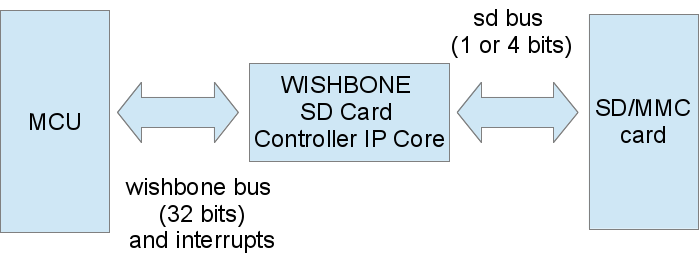
\includegraphics[width=11cm]{../bin/ip_core.png}
        % ip_core.png: 384x469 pixel, 96dpi, 10.16x12.41 cm, bb=
        \caption{SoC with SD Card IP core}
        \label{img:ip_core}
    \end{figure}
    
    \subsection{Features}
    \label{sec:fetures}
    The MMC/SD card controller provides following features:
    
    \begin{itemize}
     \item 1- or 4-bit MMC/SD mode (does not support SPI mode),
     \item 32-bit Wishbone interface,
     \item DMA engine for data transfers,
     \item Interrupt generation on completion of data and command transactions,
     \item Configurable data transfer block size,
     \item Support for any command code (including multiple data block tranfser),
     \item Support for R1, R1b, R2(136-bit), R3, R6 and R7 responses.
    \end{itemize}

\chapter{Architecture}

\section{Block diagram}
The architecture for the full IP core is shown in the Figure~\ref{blockdiagram}. It consists of 2 major parts, the actual
exponentiation core (\verb|mod_sim_exp_core| entity) with a bus interface wrapped around it. In the following sections these 
different blocks are described in detail. The bus interface and the exponentiation core can run on different clock
frequencies, so they are independent of each other.\\
\begin{figure}[H]
\centering
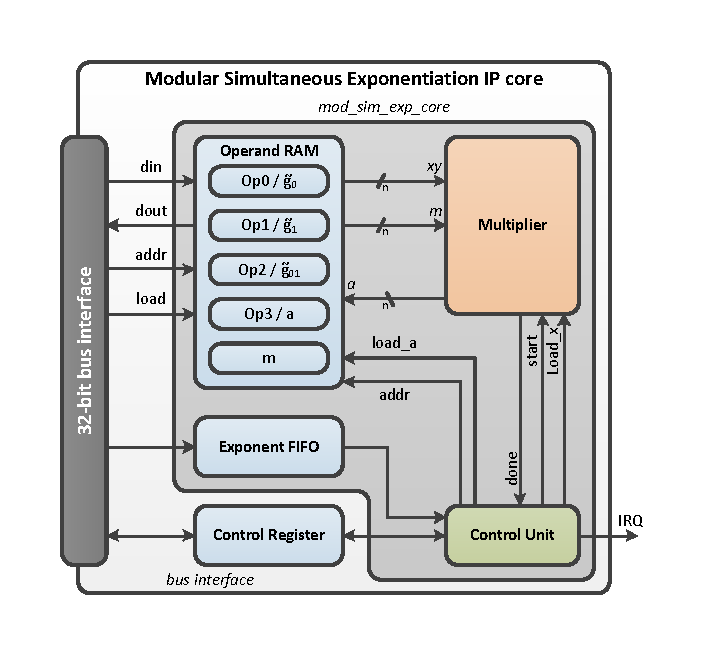
\includegraphics[trim=1.2cm 1.2cm 1.2cm 1.2cm, width=10cm]{pictures/block_diagram.pdf}
\caption{Block diagram of the Modular Simultaneous Exponentiation IP core}
\label{blockdiagram}
\end{figure}
\newpage

\section{Exponentiation core}
The exponentiation core (\verb|mod_sim_exp_core| entity) is the top level of the modular simultaneous exponentiation
core. It is made up by 4 main blocks (Figure~\ref{msec_structure}):\\

\begin{itemize}
	\item a pipelined Montgomery multiplier as the main processing unit
	\item RAM to store the operands and the modulus
	\item a FIFO to store the exponents
	\item a control unit which controls the multiplier for the exponentiation and multiplication operations
\end{itemize}

\begin{figure}[H]
\centering
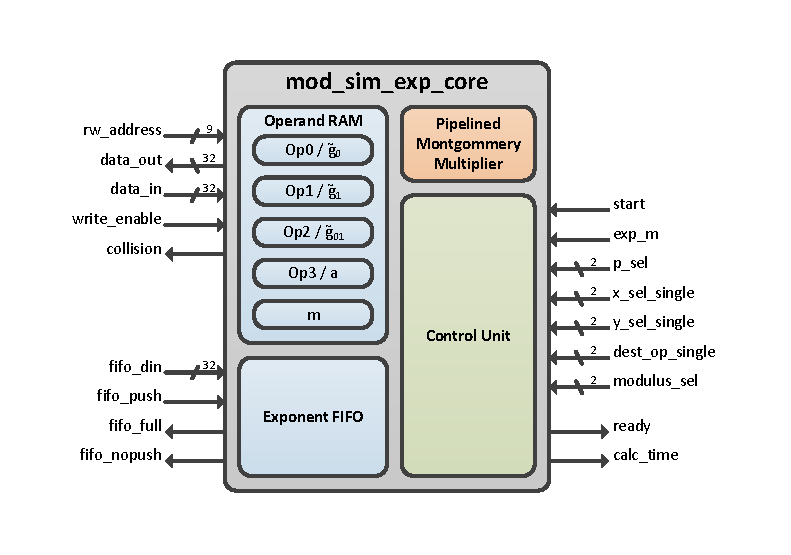
\includegraphics[trim=1.2cm 1.2cm 1.2cm 1.2cm, width=10cm]{pictures/mod_sim_exp_core.pdf}
\cprotect\caption{\verb|mod_sim_exp_core| structure}
\label{msec_structure}
\end{figure}

The multiplier and control unit operate on the \verb|core_clk| clock frequency and the interface to the operand RAM and
exponent FIFO operates on the \verb|bus_clk| clock frequency. The transition between the 2 clock domains is mainly
implemented by the RAM and FIFO. For the remainder, the necessary control signals are synchronised to the
\verb|bus_clk|. Thus when using the \verb|mod_sim_exp_core|, one can thus assume that al ports are operating on the
\verb|bus_clk| clock signal.

\subsection{Multiplier}
The kernel of this design is a pipelined Montgomery multiplier. A Montgomery multiplication\cite{MontModMul} allows efficient implementation of a
modular multiplication without explicitly carrying out the classical modular reduction step. Right-shift operations ensure that the length of the (intermediate) results does not exceed $n+1$ bits. The result of a Montgomery multiplication is given by~(\ref{eq:mont}):
\begin{align}\label{eq:mont}
r = x \cdot y \cdot R^{-1} \bmod m \hspace{1.5cm}\text{with } R = 2^{n}
\end{align}
For the structure of the multiplier, the work of \textit{Nedjah and Mourelle}\cite{NedMour} is used as a basis. They show that for large operands ($>$512 bits) the $time\times area$ product is minimal when a systolic implementation is used. This construction is composed of cells that each compute a bit of the (intermediate) result.

Because a fully unrolled two-dimensional systolic implementation would require too many resources, a systolic array (one-dimensional) implementation is chosen. This implies that the intermediate results are fed back to the same same array of cells through a register. A shift register will shift-in a bit of the $x$ operand for every step in the calculation (figure~\ref{mult_structure}). When multiplication is completed, a final check is made to ensure the result is smaller than the modulus. If not, a final reduction with $m$ is necessary.

\textbf{Note:} For this implementation the modulus $m$ has to be uneven to obtain a correct result. However, we can assume that for cryptographic applications, this is the case.


\begin{figure}[H] 
\centering 
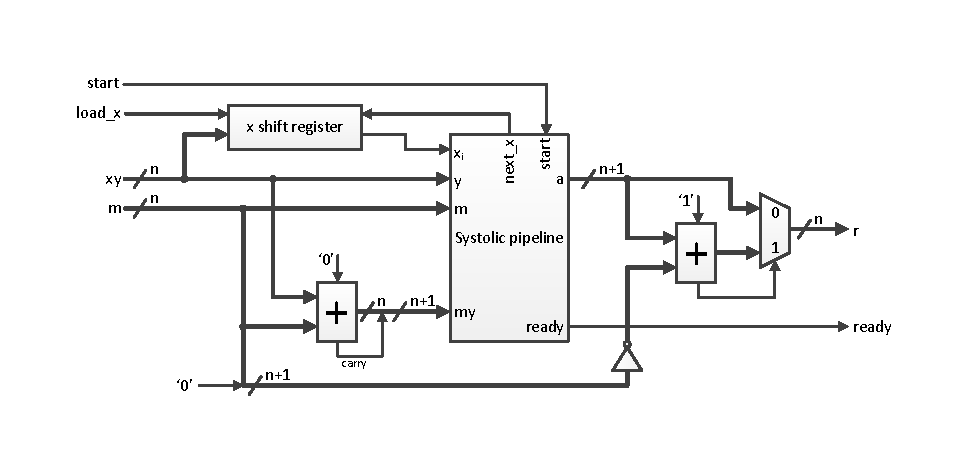
\includegraphics[trim=1.2cm 1.2cm 1.2cm 1.2cm, width=15cm]{pictures/mult_structure.pdf}
\caption{Multiplier structure. For clarification the $my$ adder and reduction logic are depicted separately, whereas in practice they are internal parts of the stages. (See Figure~\ref{stage_structure})}
\label{mult_structure}
\end{figure}

\subsubsection{Stage and pipeline structure}
The Montgomery algorithm uses a series of additions and right shifts to obtain the desired result. The main disadvantage
is the carry propagation in the adder, and therefore a pipelined version is used. The length of the operands ($n$) and
the number of pipeline stages can be chosen before synthesis. The user has the option to split the pipeline into 2
smaller parts so there are 3 operand lengths available during runtime\footnote{e.g. a total pipeline length of 1536 bit
split into a part of 512 bit and a part of 1024 bit}.

The stages and first and last cell logic design are presented in Figure~\ref{stage_structure}. Each stage takes in a
part of the modulus $m$ and $y$ operand and for each step of the multiplication, a bit of the $x$ operand is fed to the
pipeline (together with the generated $q$ signal), starting with the Least Significant Bit. The systolic array cells
need the modulus $m$, the operand $y$ and the sum $m+y$ as an input. The result from the cells is latched into a
register, and then passed back to the systolic cells for the next bit of $x$. During this pass the right shift operation
is implemented. Each stage thus needs the least significant bit from the next stage to calculate the next step. Final
reduction logic is also present in the stages for when the multiplication is complete.

An example of the standard pipeline structure is presented in Figure~\ref{pipeline_structure}. It is constructed using
stages with a predefined width. The first cell logic processes the first bit of the $m$ and $y$ operand and generates
the $q$ signal. The last cell logic finishes the reduction and selects the correct result. For operation of this
pipeline, it is clear that each stage can only compute a step every 2 clock cycles. This is because the stages rely on
the result of the next stage.

In Figure~\ref{pipeline_structure_split} an example pipeline design is drawn for a split pipeline. All multiplexers on
this figure are controlled by the pipeline select signal (\verb|p_sel|). During runtime the user can choose which part
of the pipeline is used, the lower or higher part or the full pipeline.

\newpage 
\begin{figure}[H]
\centering
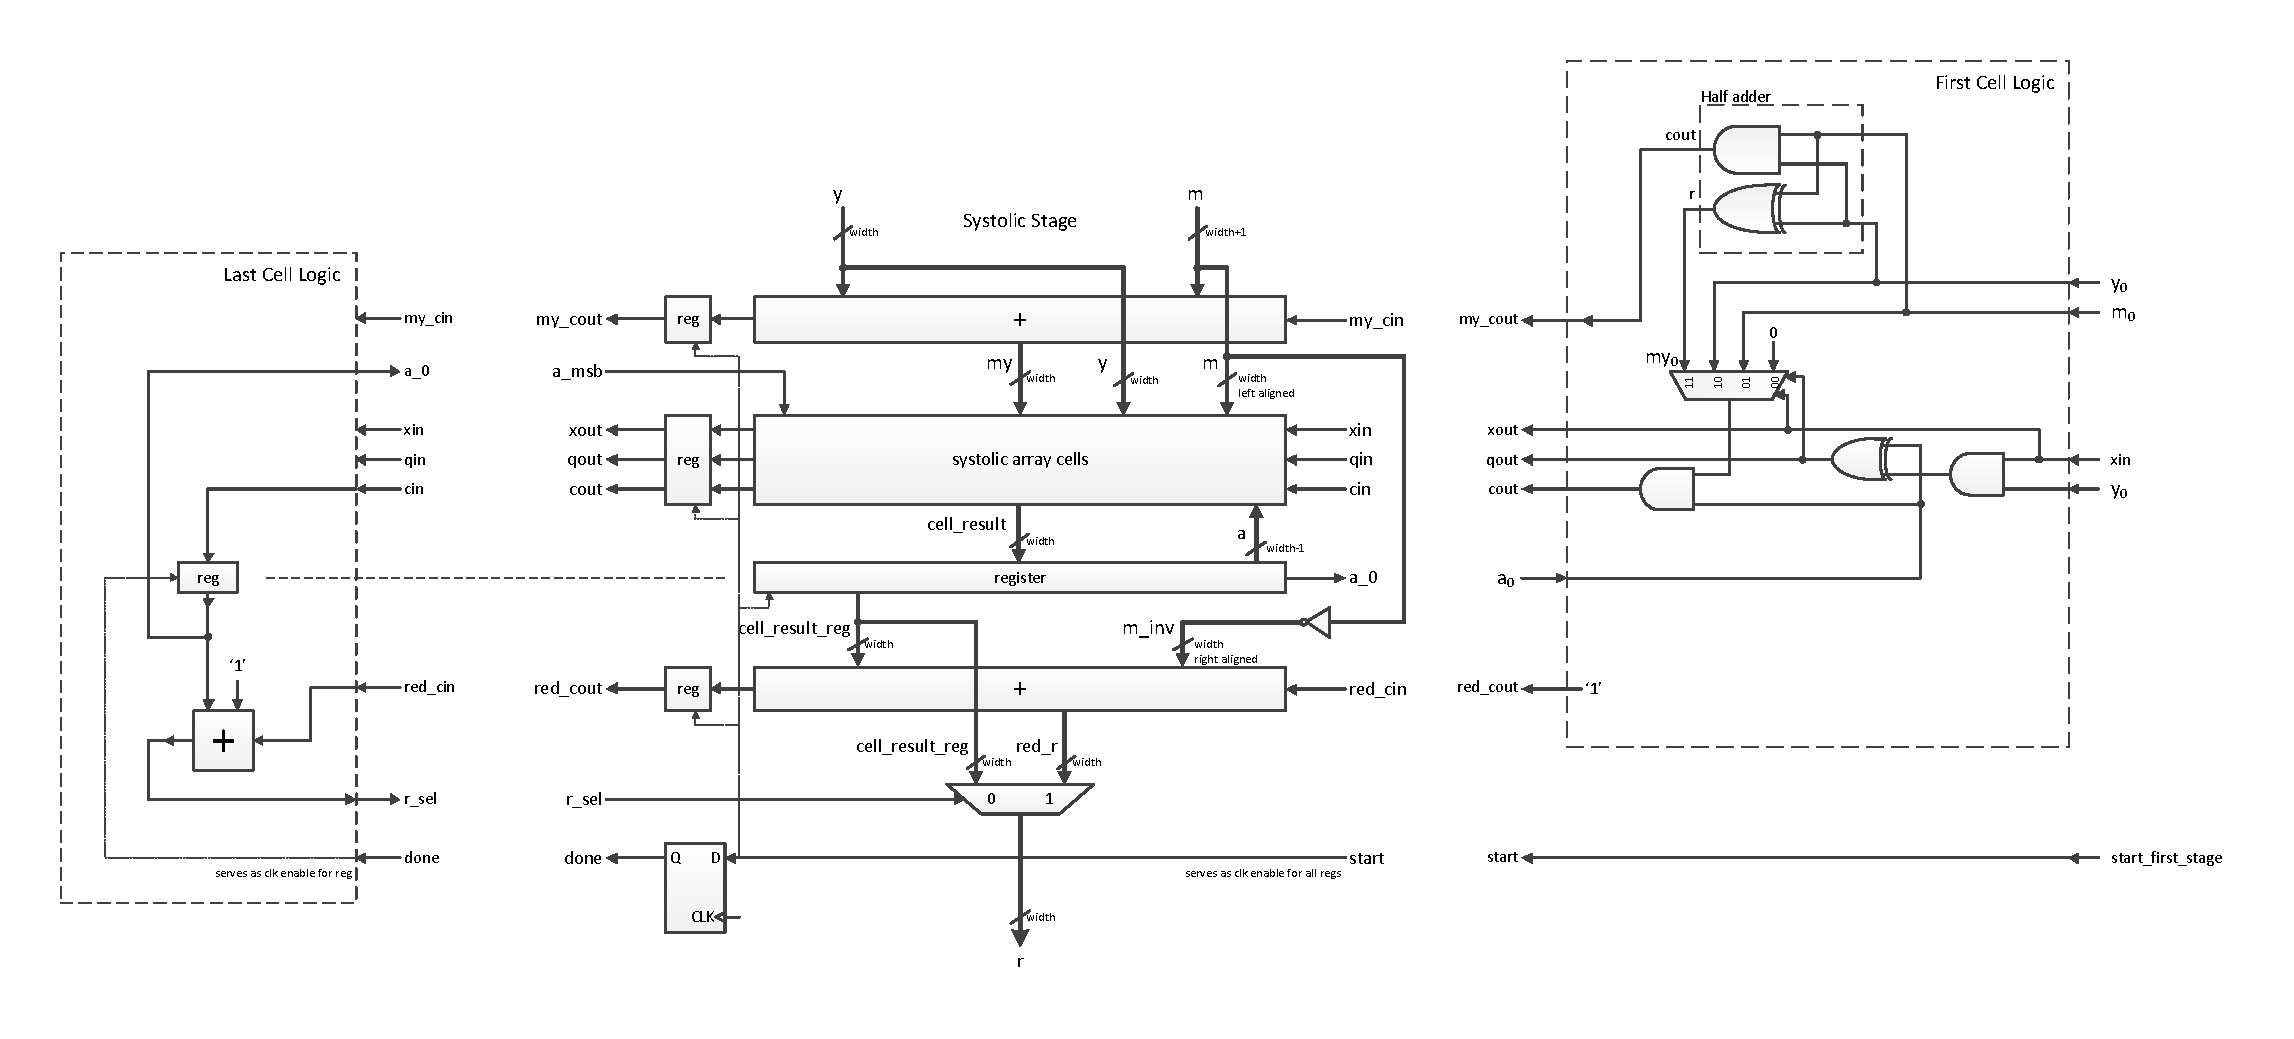
\includegraphics[trim=1.2cm 1.2cm 1.2cm 1.2cm, width=25cm, angle=90]{pictures/sys_stage.pdf}
\caption{Pipeline stage and first and last cell logic}
\label{stage_structure}
\end{figure}
\newpage

\newpage 
\begin{figure}[H]
\centering
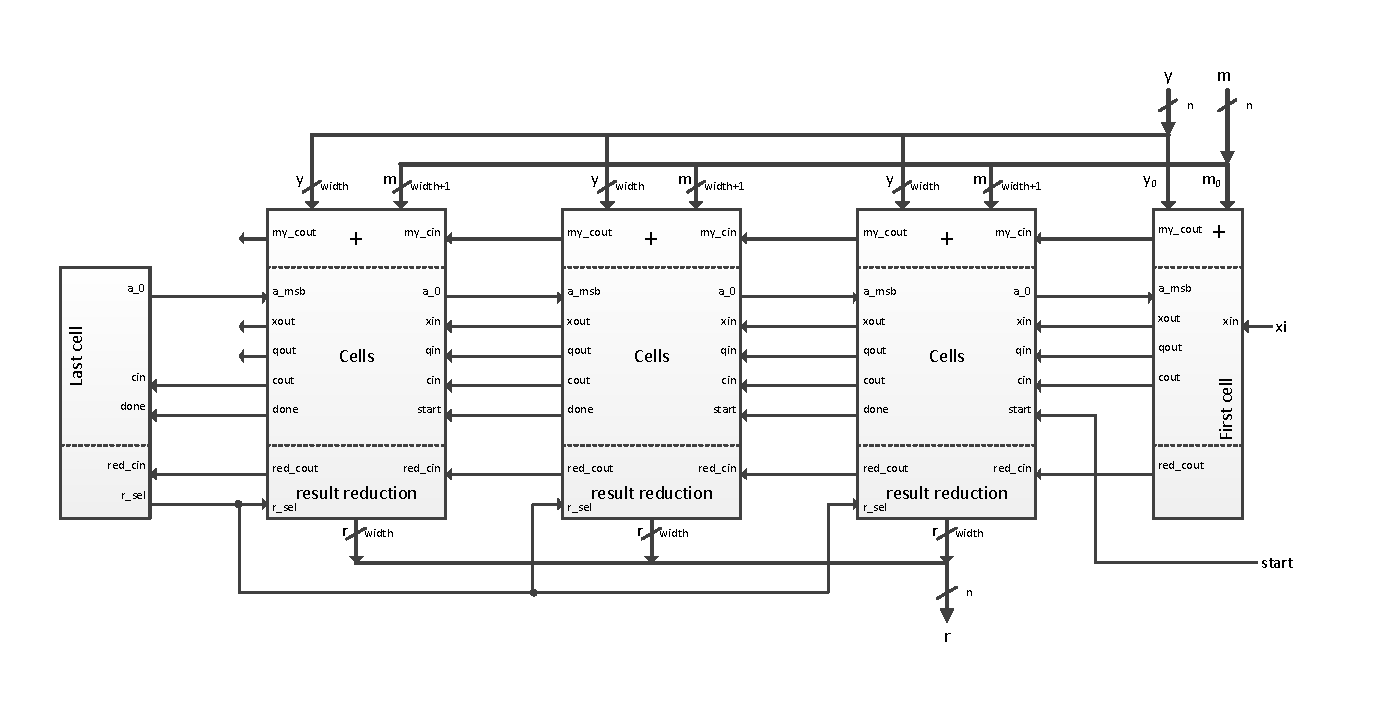
\includegraphics[trim=1.2cm 1.2cm 1.2cm 1.2cm, width=25cm, angle=90]{pictures/sys_pipeline_notsplit.pdf}
\caption{Example of the pipeline structure (3 stages)}
\label{pipeline_structure}
\end{figure}
\newpage

\newpage 
\begin{figure}[H]
\centering
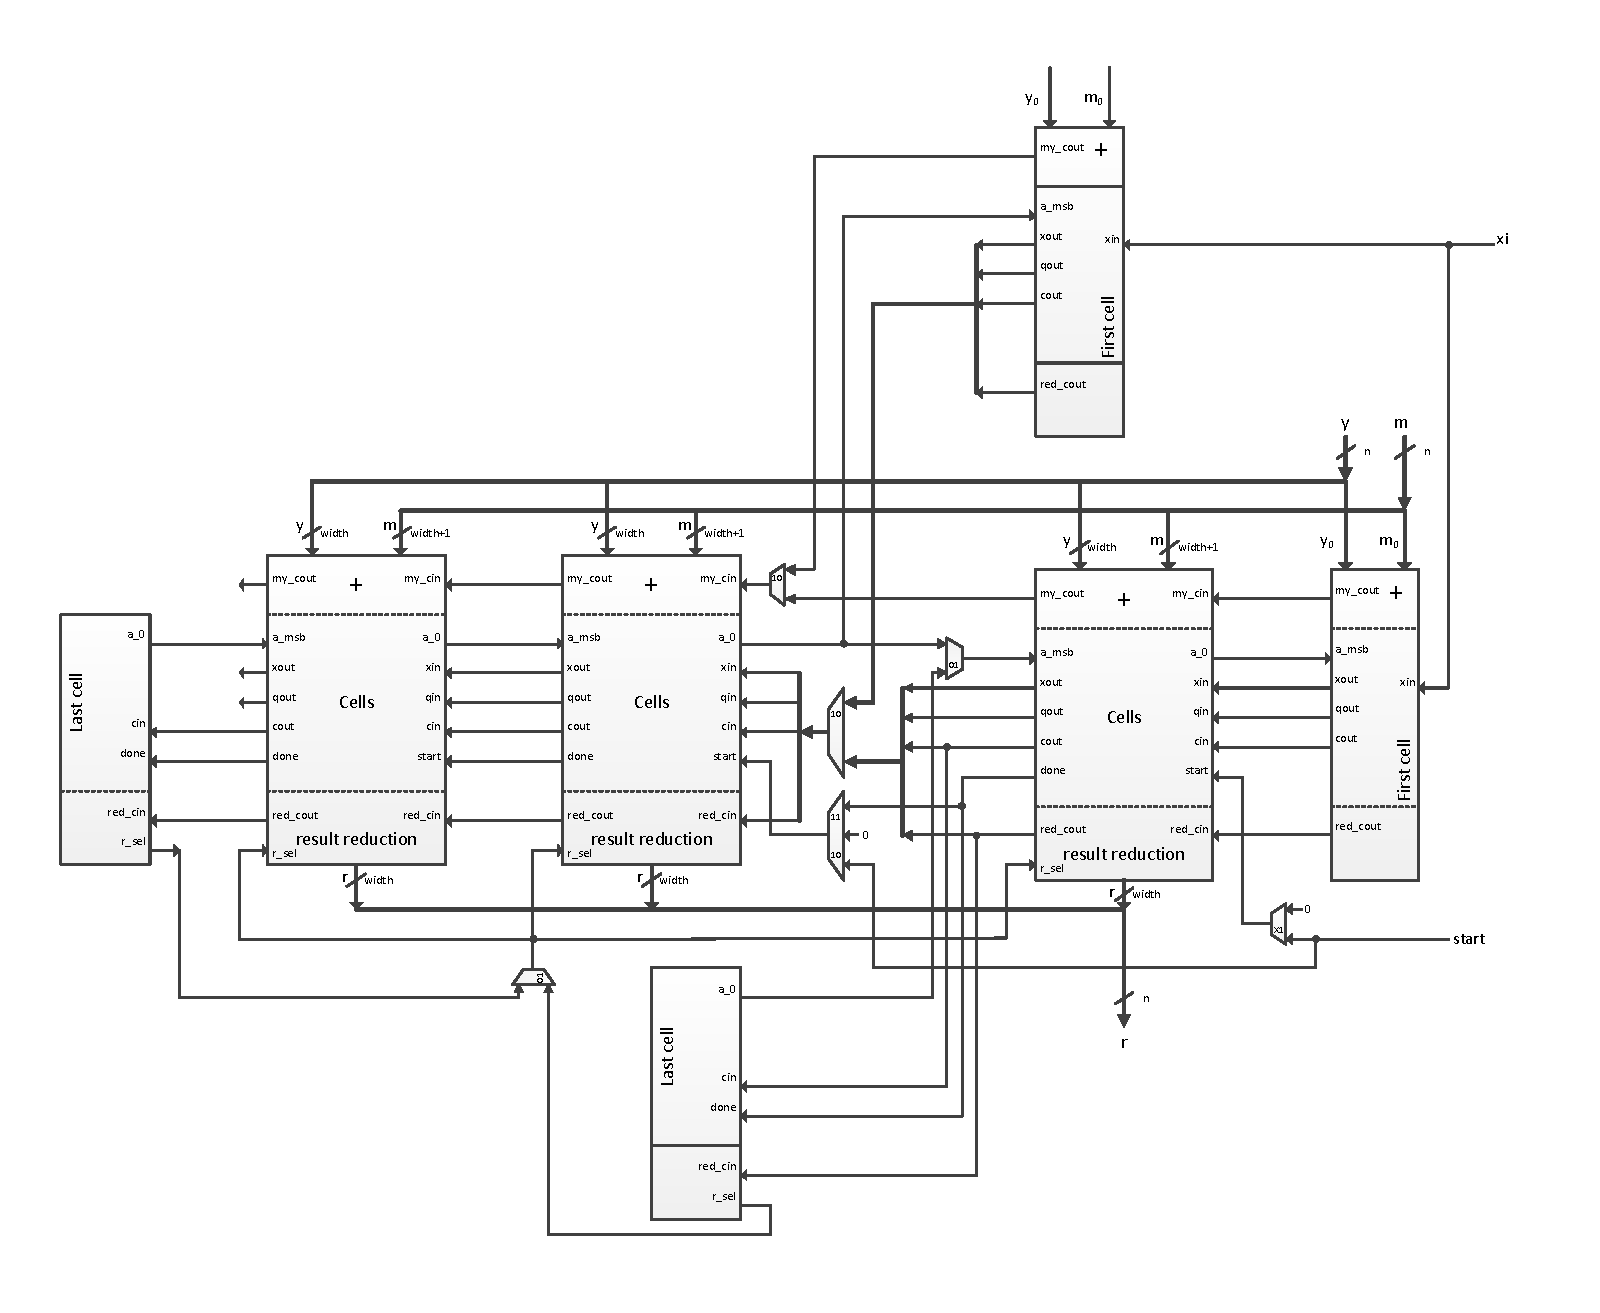
\includegraphics[trim=1.2cm 1.2cm 1.2cm 1.2cm, width=22cm, angle=90]{pictures/sys_pipeline.pdf}
\caption{Example of a split pipeline (1+2 stages)}
\label{pipeline_structure_split}
\end{figure}
\newpage


\subsection{Operand RAM and exponent FIFO} \label{subsec:RAM_and_FIFO}
The core's RAM is designed to store 4 operands and a modulus. \footnote{This is the default configuration. The number of operands can be increased, but the control logic is only designed to work with the default configuration.} Three (3) options are available for the implementation of the RAM. Setting the parameter \verb|C_MEM_STYLE|, will change the implementation style. All styles try to use the RAM resources available on the FPGA.

If the FPGA supports asymmetric RAMs, i.e. with a different read and write width, we suggest that the option \verb|"asym"| is selected. Since the (device specific) RAM blocks are inferred through code, it is imperative to select the right device (\verb|C_FPGA_MAN|), as this inference is different between manufacturers. Currently, only Altera and Xilinx are supported.

If there's no asymmetric RAM support, the option \verb|"generic"| should be selected. This option will work for most FPGAs, but the disadvantage is that it will use more resources than the \verb|"asym"| option. This is because a significant number of LUTs will be used to construct an asymmetric RAM.

For both options the size of the RAM adapts dynamically to the chosen pipeline width (\verb|C_NR_BITS_TOTAL|).

Finally, the option \verb|"xil_prim"| is targeted specifically to Xilinx devices. It uses blocks of RAM generated with CoreGen. These blocks are of a fixed width and this results in a fixed RAM of 4x1536 bit for the operands and 1536 bit for the modulus. This option is deprecated in favor of \verb|"asym"|.

Reading and writing (from the bus side) to the operands and modulus is done one 32-bit word at a time. If using a split pipeline, it is important that operands for the higher part of the pipeline are loaded into the RAM with preceding zero's for the lower bits of the pipeline. As a rule of thumb, the number of FPGA RAM blocks that will be used is given by (\ref{eq:ramblocks}):
\begin{align}
	2 \cdot \mathtt{C\_NR\_BITS\_TOTAL} / 32\label{eq:ramblocks}
\end{align}
\newline

To store the exponents, there is a FIFO of 32 bit wide. Every 32 bit entry has to be formatted as 16 bit of $e_0$ for the
lower part [15:0] and 16 bit of $e_1$ for the higher part [31:16]. Entries have to be pushed in the FIFO starting with the least significant word and ending with the most significant word of the exponents.

For the FIFO there are 2 styles available. The implementation style depends on the style of the operand memory and it can not be set directly. When the RAM option \verb|"xil_prim"| is chosen, the resulting FIFO will use the FIFO18E1 primitive. It is able to store 512 entries, meaning 2 exponents of each 8192 bit long.

When the RAM options \verb|"generic"| or \verb|"asym"| are chosen, a generic FIFO \footnote{This FIFO is a slightly
modified version of the generic FIFOs project at OpenCores.org (http://opencores.org/project,generic\_fifos).} will be
implemented.
This consist of a dual port symmetric RAM with the control logic for a FIFO. The depth of this generic FIFO is adjustable with the parameter \verb|C_FIFO_AW|. The number of RAM blocks for the FIFO is given by (\ref{eq:fifoblocks}), where
\verb|RAMBLOCK_SIZE| is the size [bits] of the FPGA's RAM primitive.
\begin{align}
	\left[\left(\mathtt{2^{C\_FIFO\_AW}}+1\right) \cdot 32 \right]/ \mathtt{RAMBLOCK\_SIZE} \label{eq:fifoblocks}
\end{align}

\subsection{Control unit}
The control unit loads in the operands and has full control over the multiplier. For single multiplications, it latches in 
the $x$ operand, then places the $y$ operand on the bus and starts the multiplier. In case of an exponentiation, the FIFO is 
emptied while the necessary single multiplications are performed. When the computation is done, the ready signal is 
asserted to notify the system.

\newpage
\subsection{IO ports and memory map}
The \verb|mod_sim_exp_core| IO ports\\
\newline
% Table generated by Excel2LaTeX
\begin{tabular}{|l|c|c|p{8cm}|}
\hline
\rowcolor{Gray}
\textbf{Port} & \textbf{Width} & \textbf{Direction} & \textbf{Description} \bigstrut\\
\hline
\verb|core_clk|   & 1     & in    & core clock input, clock signal for the multiplier and control unit \bigstrut\\
\hline
\verb|bus_clk|   & 1     & in    & bus clock input, clock signal for all core IO \bigstrut\\
\hline
\verb|reset| & 1     & in    & reset signal (active high) resets the pipeline, fifo and control logic \bigstrut\\
\hline
\multicolumn{4}{|l|}{\textbf{\textit{operand memory interface}}} \bigstrut\\
\hline
\verb|rw_address| & 9     & in    & operand memory read/write address (structure descibed below) \bigstrut\\
\hline
\verb|data_out| & 32    & out   & operand data out (0 is lsb) \bigstrut\\
\hline
\verb|data_in| & 32    & in    & operand data in (0 is lsb) \bigstrut\\
\hline
\verb|write_enable| & 1     & in    & write enable signal, latches \verb|data_in| to operand RAM \bigstrut\\
\hline
\verb|collision| & 1     & out   & collision output, asserts on a write error \bigstrut\\
\hline
\multicolumn{4}{|l|}{\textbf{\textit{exponent FIFO interface}}} \bigstrut\\
\hline
\verb|fifo_din| & 32    & in    & FIFO data in, bits [31:16] for $e_1$ operand and bits [15:0] for $e_0$ operand \bigstrut\\
\hline
\verb|fifo_push| & 1     & in    & push \verb|fifo_din| into the FIFO \bigstrut\\
\hline
\verb|fifo_nopush| & 1     & out   & flag to indicate if there was an error pushing the word to the FIFO \bigstrut\\
\hline
\verb|fifo_full| & 1     & out   & flag to indicate the FIFO is full \bigstrut\\
\hline
\multicolumn{4}{|l|}{\textbf{\textit{control signals}}} \bigstrut\\
\hline
\verb|x_sel_single| & 2     & in    & selection for x operand source during single multiplication \bigstrut\\
\hline
\verb|y_sel_single| & 2     & in    & selection for y operand source during single multiplication \bigstrut\\
\hline
\verb|dest_op_single| & 2     & in    & selection for the result destination operand for single multiplication \bigstrut\\
\hline
\verb|p_sel| & 2     & in    & specifies which pipeline part to use for exponentiation / multiplication. \bigstrut[t]\\
      &       &       & ``01'' : use lower pipeline part \\
      &       &       & ``10'' : use higher pipeline part \\
      &       &       & ``11'' : use full pipeline \bigstrut[b]\\
\hline
\verb|modulus_sel| & 1     & in    & selection for which modulus to use for the calculations (only available if \verb|C_MEM_STYLE| = \verb|"generic"| or \verb|"asym"|). Otherwise set to 0 \bigstrut\\
\hline
\verb|exp_m| & 1     & in    & core operation mode. ``0'' for single multiplications and ``1'' for exponentiations \bigstrut\\
\hline
\verb|start| & 1     & in    & start the calculation for current mode \bigstrut\\
\hline
\verb|ready| & 1     & out   & indicates the multiplication/exponentiation is done \bigstrut\\
\hline
\verb|calc_time| & 1     & out   & is high during a multiplication, indicator for used calculation time \bigstrut\\
\hline
\end{tabular}%
\newpage
The \verb|mod_sim_exp_core| parameters\\
\begin{center}
	\begin{tabular}{|l|p{6.5cm}|c|l|}
		\hline
		\rowcolor{Gray}
		\textbf{Name} & \textbf{Description} & \textbf{VHDL Type} &\textbf{Default Value} \bigstrut\\
		\hline
		\verb|C_NR_BITS_TOTAL| & total width of the multiplier in bits & integer & 1536\bigstrut\\
		\hline
		\verb|C_NR_STAGES_TOTAL| & total number of stages in the pipeline & integer & 96\bigstrut\\
		\hline
		\verb|C_NR_STAGES_LOW| & number of lower stages in the pipeline, defines the bit-width of the lower pipeline part & integer & 32 \bigstrut\\
		\hline
		\verb|C_SPLIT_PIPELINE| & option to split the pipeline in 2 parts & boolean & true \bigstrut\\
		\hline
		\verb|C_FIFO_AW| & address width of the generic FIFO pointers, FIFO size is equal to $2^{C\_FIFO\_AW} $. & integer & 7 \bigstrut\\
						 & only	applicable if \verb|C_MEM_STYLE| = \verb|"generic"| or \verb|"asym"|  & & \\
		\hline
		\verb|C_MEM_STYLE| & select the RAM memory style (3 options): & string & \verb|"generic"| \bigstrut\\
							& \verb|"generic"| : use general 32-bit RAMs & & \\
      						& \verb|"asym"| : use asymmetric RAMs & & \\
      						& (For more information see \ref{subsec:RAM_and_FIFO}) & & \\
      						& \verb|"xil_prim"| : use xilinx primitives & &\\
      						& (deprecated) & & \bigstrut[b] \\
		\hline
		\verb|C_FPGA_MAN| & device manufacturer: & & \\
						& \verb|"xilinx"| or \verb|"altera"| & string & \verb|"xilinx"| \bigstrut\\
		\hline
	\end{tabular}%
\end{center}

The following figure describes the structure of the Operand RAM memory, for every operand there is a space of 2048 bits 
reserved. So operand widths up to 2048 bits are supported.\\
\newline \\
\begin{figure}[H]
\centering
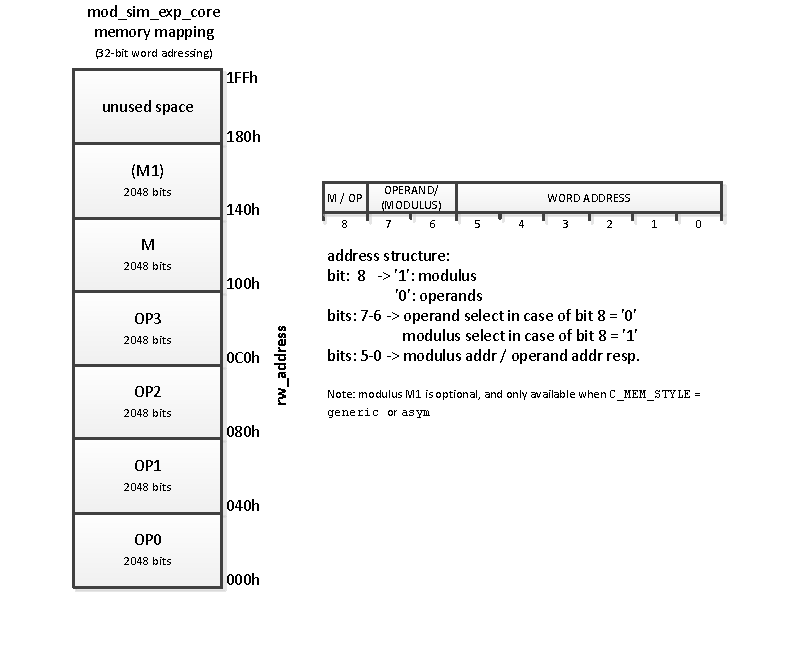
\includegraphics[trim=1.2cm 1.2cm 1.2cm 1.2cm, width=15cm]{pictures/msec_memory.pdf}
\caption{Address structure of the exponentiation core}
\label{Address_structure}
\end{figure}

\section{Bus interface}
The bus interface implements the register necessary for the control unit inputs to the \verb|mod_sim_exp_core| entity.
It also maps the memory to the required bus and connects the interrupt signals. The embedded processor then has full control
over the core.
\chapter{Operation}

\section{Pipeline operation}
The operation of the pipeline is shown in Figure~\ref{fig:pipeline_op}. One can see that the stages are started
every 2 clock cycles ($\tau_{c}$ is the core clock period). This is needed because the least significant bit of the next
stage result is needed. Every stage has to run $n$ (the width of the operands) times for the multiplication to be complete.

\begin{figure}[H]	
\centering
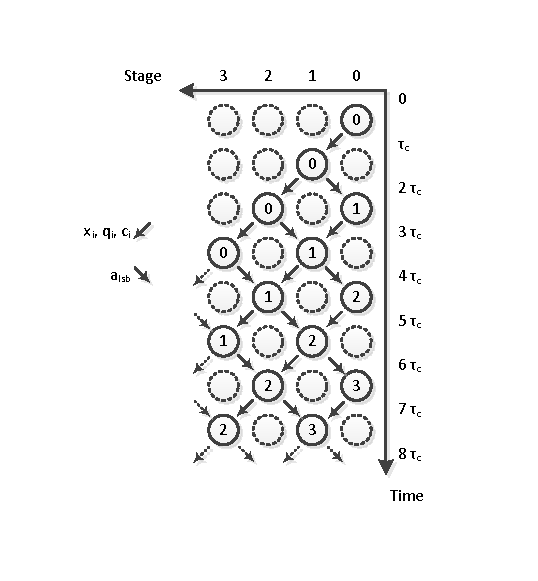
\includegraphics[trim=1.2cm 1.2cm 1.2cm 1.2cm, width=7cm]{pictures/pipeline_operation.pdf}
\caption{Pipeline operation: Each circle represents an active stage. The number indicates how much times that stage 
		has run. Dotted line contours indicate the stage is inactive.}
\label{fig:pipeline_op}
\end{figure}

For performing one Montgomery multiplication using this core, the total computation time $T_m$ for an $n$-bit operand
with a $k$-stage pipeline is given by~(\ref{eq:Tmult}).
\begin{align}\label{eq:Tmult}
T_{m} = \left[k + 2(n - 1)\right] \tau_c
\end{align}
\newpage
\section{Modular Simultaneous exponentiation operations}
Exponentiations are calculated with Algorithm~\ref{alg:mme} which uses the Montgomery multiplier as the main computation
step. It uses the principle of a square-and-multiply algorithm to calculate an exponentiation with 2 bases.
\begin{algorithm}[H] % enter the algorithm environment
\caption{Montgomery simultaneous exponentiation} % give the algorithm a caption
\label{alg:mme} % and a label for \ref{} commands later in the document
\algnewcommand\algorithmicdownto{\textbf{downto}}
\algrenewtext{For}[3]%
{\algorithmicfor\ #1 $\gets$ #2 \algorithmicdownto\ #3 \algorithmicdo}
\algnewcommand\algorithmicswitch{\textbf{switch}}
\algrenewtext{While}[2]%
{\algorithmicswitch\ #1, #2}
\algnewcommand\algorithmicinput{\textbf{Input:}}
\algnewcommand\Input{\item[\algorithmicinput]}
\algnewcommand\algorithmicoutput{\textbf{Output:}}
\algnewcommand\Output{\item[\algorithmicoutput]}
\footnotesize
\begin{algorithmic}[1] % enter the algorithmic environment
\Input $g_{0},\:g_{1},\:e_{0}=(e_{0_{t-1}} \cdots e_{0_{0}})_{2},\:e_{1}=(e_{0_{t-1}} \cdots e_{0_{0}})_{2},\:R^{2}\bmod m,\:m$
\Output $g_{0}^{e_{0}} \cdot g_{1}^{e_{1}} \bmod m$
\State $\tilde{g}_{0} := \text{Mont}(g_{0}, R^{2}),\:\tilde{g}_{1} := \text{Mont}(g_{1}, R^{2}),\:\tilde{g}_{01} := \text{Mont}(\tilde{g}_{0}, \tilde{g}_{1})$
\State $a := \text{Mont}(R^{2}, 1)$
\Comment This is the same as $a := R \bmod m$.
\For{$i$}{$(t-1)$}{0}
\State $a := \text{Mont}(a, a)$
\While{$e_{1_{i}}$}{$e_{0_{i}}$} % use as switch statement
\State $0,\:1:\;a := \text{Mont}(a, \tilde{g}_{0})$
\State $1,\:0:\;a := \text{Mont}(a, \tilde{g}_{1})$
\State $1,\:1:\;a := \text{Mont}(a, \tilde{g}_{01})$
\EndWhile
\EndFor
\State $a := \text{Mont}(a, 1)$
\State \Return{$a$}
\end{algorithmic}
\end{algorithm}
It can be seen that the algorithm requires $R^{2}\bmod m$ which is $2^{2n}\bmod m$. We assume $R^2 \bmod m$ can be
provided or pre-computed. The for loop in the algorithm is executed by the control logic of the core. Apart from this,
a few pre- and one post-calculations have to be performed.

The computation time for an exponentiation depends on the number of zero's in the exponents, from
Algorithm~\ref{alg:mme} one can see that if both exponent bits are zero at a time, no multiplication has to be
performed. Thus reducing the total time. The average computation time for a modular simultaneous exponentiation, with
$n$-bit base operands and $t$-bit exponents is given by~(\ref{eq:Tsime}).
\begin{align}\label{eq:Tsime}
T_{se} = \frac{7}{4} t \cdot T_{m} = \frac{7}{4}t \cdot [k + 2(n - 1)] \tau_c 
\end{align}

For single base exponentiations, i.e. 1 exponent is equal to zero, the average exponentiation time is given by~(\ref{eq:Texp}).
\begin{align}\label{eq:Texp}
T_{e} = \frac{3}{2} t \cdot T_{m} = \frac{3}{2}t \cdot [k + 2(n - 1)] \tau_c 
\end{align}

The formulas~(\ref{eq:Tsime}) and~(\ref{eq:Texp}) given here are only the theoretical average time for an exponentiation,
excluding the pre- and post-computations.


\section{Core operation steps}
The core can operate in 2 modes, multiplication or exponentiation mode. The steps required to do one of these actions
are described here.
\subsection{Single Montgomery multiplication}
The following steps are needed for a single Montgomery multiplication:
\begin{enumerate}
  	\item load the modulus to the RAM using the 32 bit bus
	\item load the desired $x$ and $y$ operands into any 2 locations of the operand RAM using the 32 bit bus.
	\item select the correct input operands for the multiplier using \verb|x_sel_single| and \verb|y_sel_single|
	\item select the result destination operand using \verb|result_dest_op|
	\item set \verb|exp/m| = `0' to select multiplication mode
	\item set \verb|p_sel| to choose which pipeline part you will use
	\item generate a start pulse for the core
	\item wait until interrupt is received and read out result in selected operand
\end{enumerate}

\textbf{Note:} this computation gives a result \( r = x \cdot y \cdot R^{-1} \bmod m\). If the actual product of $x$ and $y$ is
desired, a final Montgomery multiplication of the result with $R^{2}$ is needed.

\subsection{Modular simultaneous exponentiation}
The core requires $\tilde{g}_{0}$, $\tilde{g}_{0}$, $\tilde{g}_{01}$ and $a$ to be loaded into the correct operand
spaces before starting the exponentiation. These parameters are calculated using single Montgomery multiplications as follows:
\begin{align*}
	\tilde{g}_{0} &= Mont(g_{0}, R^{2}) &\,&= g_{0} \cdot R \bmod m & \hspace{3cm}\text{in operand 0}\hspace{4cm}\\
	\tilde{g}_{1} &= Mont(g_{1}, R^{2}) &\,&= g_{1} \cdot R \bmod m & \hspace{3cm}\text{in operand 1}\hspace{4cm}\\
	\tilde{g}_{01} &= Mont(\tilde{g}_{0}, \tilde{g}_{1}) &\,&= g_{0} \cdot g_{1} \cdot R \bmod m & \hspace{3cm}\text{in operand 2}\hspace{4cm}\\
	a &= Mont(R^{2}, 1) &\,&= R \bmod m &\hspace{3cm}\text{in operand 3}\hspace{4cm}
\end{align*}
When the exponentiation is done, a final multiplication has to be started by the software to multiply $a$ with 1.
The steps needed for a full simultaneous exponentiation are:


\begin{enumerate}
  	\item load the modulus to the RAM using the 32 bit bus
	\item load the desired $g_0$, $g_1$ operands and \(R^{2} \bmod m\) into the operand RAM using the 32 bit bus.
	\item set \verb|p_sel| to choose which pipeline part you will use
	\item compute $\tilde{g}_{0}$ by using a single Montgomery multiplication of $g_{0}$ with $R^{2}$ and place the result $\tilde{g}_{0}$ in operand 0.
	\item compute $\tilde{g}_{1}$ by using a single Montgomery multiplication of $g_{1}$ with $R^{2}$ and place the result $\tilde{g}_{1}$ in operand 1.
	\item compute $\tilde{g}_{01}$ by using a single Montgomery multiplication of $\tilde{g}_{0}$ with $\tilde{g}_{1}$ and place the result $\tilde{g}_{01}$ in operand 2.
	\item compute $a$ by using a single Montgomery multiplication of $R^{2}$ with $1$ and place the result $a$ in operand 3.
	\item set the core in exponentiation mode ($exp/m$='1')
	\item generate a start pulse for the core
	\item wait until interrupt is received
	\item perform the post-computation using a single Montgomery multiplication of $a$(in operand 3) with 1 and read out result
\end{enumerate}
\chapter{PLB interface}
\section{Structure}
The Processor Local Bus interface for this core is structured as in Figure~\ref{PLBstructure}. The core acts as a slave
to the PLB bus. The PLB v4.6 Slave\cite{XilinxPLB} logic translates the interface to a lower level IP Interconnect
Interface (IPIC).
This is then used to connect the core internal components to. The user logic contains the exponentiation core and the
control register for the core its control inputs and outputs. An internal interrupt controller\cite{XilinxIntr} handles
the outgoing interrupt requests and a software reset module is provided to be able to reset the IP core at runtime. This
bus interface is created using the ``Create or Import Peripheral'' wizard from Xilinx Platform Studio.\\
\begin{figure}[H]	
\centering
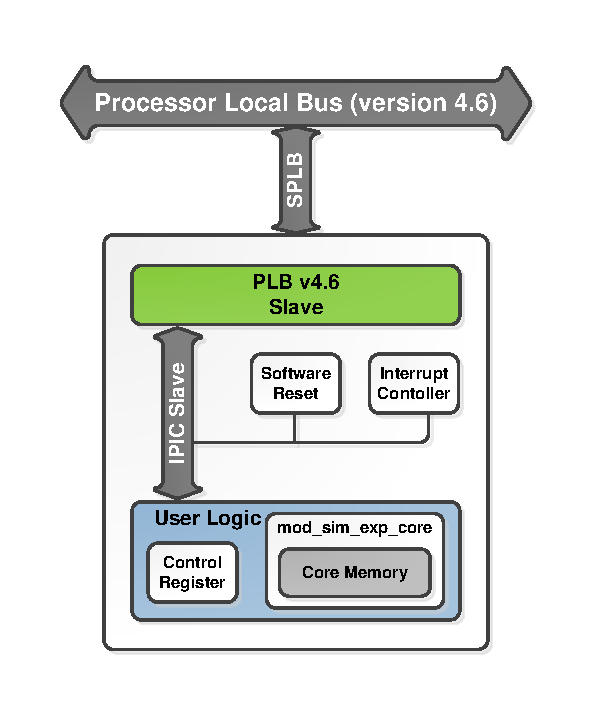
\includegraphics[trim=1.2cm 1.2cm 1.2cm 1.2cm, width=7cm]{pictures/plb_interface.pdf}
\caption{PLB IP core structure}
\label{PLBstructure}
\end{figure}

\newpage
\section{Parameters}
This section describes the parameters used to configure the core, only the relevant parameters are discussed. PLB
specific parameters are left to the user to configure. The IP core specific parameters and their respective use are
listed in the table below.
\begin{center}
	\begin{tabular}{|l|p{6.5cm}|c|l|}
		\hline
		\rowcolor{Gray}
		\textbf{Name} & \textbf{Description} & \textbf{VHDL Type} &\textbf{Default Value} \bigstrut\\
		\hline
		\multicolumn{4}{|l|}{\textit{\textbf{Memory configuration}}} \\		
		\hline
		\verb|C_FIFO_AW| & address width of the generic FIFO pointers, FIFO size is equal to $2^{C\_FIFO\_AW} $. & integer & 7 \bigstrut\\
						 & only	applicable if \verb|C_MEM_STYLE| = \verb|"generic"| or \verb|"asym"|  & & \\
		\hline
		\verb|C_MEM_STYLE| & the memory structure to use for the RAM, choice between 3 options: & string & \verb|"generic"| \bigstrut\\
							& \verb|"xil_prim"| : use xilinx primitives & & \\
      						& \verb|"generic"| : use general 32-bit RAMs & & \\
      						& \verb|"asym"| : use asymmetric RAMs & & \\
      						& (For more information see \ref{subsec:RAM_and_FIFO}) & & \bigstrut[b] \\
		\hline
		\verb|C_FPGA_MAN| & device manufacturer: & string & \verb|"xilinx"| \\
						& \verb|"xilinx"| or \verb|"altera"| &  &  \bigstrut\\
		\hline
		\verb|C_BASEADDR| & base address for the IP core's memory space & std\_logic\_vector & X"FFFFFFFF" \bigstrut\\
		\hline
		\verb|C_HIGHADDR| & high address for the IP core's memory space & std\_logic\_vector & X"00000000" \bigstrut\\
		\hline
		\verb|C_M_BASEADDR| & base address for the modulus memory space & std\_logic\_vector & X"FFFFFFFF" \bigstrut\\
		\hline
		\verb|C_M_HIGHADDR| & high address for the modulus memory space & std\_logic\_vector & X"00000000" \bigstrut\\
		\hline
		\verb|C_OP0_BASEADDR| & base address for the operand 0 memory space & std\_logic\_vector & X"FFFFFFFF" \bigstrut\\
		\hline
		\verb|C_OP0_HIGHADDR| & high address for the operand 0 memory space & std\_logic\_vector & X"00000000" \bigstrut\\
		\hline
		\verb|C_OP1_BASEADDR| & base address for the operand 1 memory space & std\_logic\_vector & X"FFFFFFFF" \bigstrut\\
		\hline
		\verb|C_OP1_HIGHADDR| & high address for the operand 1 memory space & std\_logic\_vector & X"00000000" \bigstrut\\
		\hline
		\verb|C_OP2_BASEADDR| & base address for the operand 2 memory space & std\_logic\_vector & X"FFFFFFFF" \bigstrut\\
		\hline
		\verb|C_OP2_HIGHADDR| & high address for the operand 2 memory space & std\_logic\_vector & X"00000000" \bigstrut\\
		\hline
		\verb|C_OP3_BASEADDR| & base address for the operand 3 memory space & std\_logic\_vector & X"FFFFFFFF" \bigstrut\\
		\hline
		\verb|C_OP3_HIGHADDR| & high address for the operand 3 memory space & std\_logic\_vector & X"00000000" \bigstrut\\
		\hline
		\verb|C_FIFO_BASEADDR| & base address for the FIFO memory space & std\_logic\_vector & X"FFFFFFFF" \bigstrut\\
		\hline
		\verb|C_FIFO_HIGHADDR| & high address for the FIFO memory space & std\_logic\_vector & X"00000000" \bigstrut\\
		\hline
		\multicolumn{4}{|l|}{\textit{\textbf{Multiplier configuration}}} \\
		\hline
		\verb|C_NR_BITS_TOTAL| & total width of the multiplier in bits & integer & 1536\bigstrut\\
		\hline
		\verb|C_NR_STAGES_TOTAL| & total number of stages in the pipeline & integer & 96\bigstrut\\
		\hline
		\verb|C_NR_STAGES_LOW| & number of lower stages in the pipeline, defines the bit-width of the lower pipeline part & integer & 32 \bigstrut\\
		\hline
		\verb|C_SPLIT_PIPELINE| & option to split the pipeline in 2 parts & boolean & true \bigstrut\\
		\hline
	\end{tabular}%
\end{center}
%\newline 

The complete IP core's memory space can be controlled. As can be seen, the operand, modulus and FIFO memory space can be
chosen separately from the IP core's memory space which hold the registers for control, software reset and interrupt
control. The core's memory space must have a minimum width of 1K byte for all registers to be accessible. For the FIFO
memory space, a minimum width of 4 byte is needed, since the FIFO is only 32 bit wide. The memory space width for the
operands and the modulus need a minimum width equal to the total multiplier width.\\

There are 4 parameters to configure the multiplier. These values define the width of the multiplier operands and the
number of pipeline stages. If \verb|C_SPLIT_PIPELINE| is false, only operands with a width of\\\verb|C_NR_BITS_TOTAL| are
valid. Else if \verb|C_SPLIT_PIPELINE| is true, 3 operand widths can be supported:
\begin{itemize}
  \item the length of the full pipeline ($C\_NR\_BITS\_TOTAL$)
  \item the length of the lower pipeline ($\frac{C\_NR\_BITS\_TOTAL}{C\_NR\_STAGES\_TOTAL} \cdot C\_NR\_STAGES\_LOW $)
  \item the length of the higher pipeline ($\frac{C\_NR\_BITS\_TOTAL}{C\_NR\_STAGES\_TOTAL} \cdot (C\_NR\_STAGES\_TOTAL - C\_NR\_STAGES\_LOW$)
\end{itemize}

\section{IO ports}
\begin{tabular}{|l|c|c|l|}
	\hline
	\rowcolor{Gray}
	\textbf{Port} & \textbf{Width} & \textbf{Direction} & \textbf{Description} \\
	\hline
	\multicolumn{4}{|l|}{\textit{\textbf{PLB bus connections}}} \\
	\hline
	\verb|SPLB_Clk| & 1     & in & see note 1 \\
	\hline
	\verb|SPLB_Rst| & 1     & in & see note 1 \\
	\hline
	\verb|PLB_ABus| & 32    & in & see note 1 \\
	\hline
	\verb|PLB_PAValid| & 1     & in & see note 1 \\
	\hline
	\verb|PLB_masterID| & 3     & in & see note 1 \\
	\hline
	\verb|PLB_RNW| & 1     & in & see note 1 \\
	\hline
	\verb|PLB_BE| & 4     & in & see note 1 \\
	\hline
	\verb|PLB_size| & 4     & in & see note 1 \\
	\hline
	\verb|PLB_type| & 3     & in & see note 1 \\
	\hline
	\verb|PLB_wrDBus| & 32    & in & see note 1 \\
	\hline
	\verb|Sl_addrAck| & 1     & out & see note 1 \\
	\hline
	\verb|Sl_SSize| & 2     & out & see note 1 \\
	\hline
	\verb|Sl_wait| & 1     & out & see note 1 \\
	\hline
	\verb|Sl_rearbitrate| & 1     & out & see note 1 \\
	\hline
	\verb|Sl_wrDack| & 1     & out & see note 1 \\
	\hline
	\verb|Sl_wrComp| & 1     & out & see note 1 \\
	\hline
	\verb|Sl_rdBus| & 32    & out & see note 1 \\
	\hline
	\verb|Sl_MBusy| & 8     & out & see note 1 \\
	\hline
	\verb|Sl_MWrErr| & 8     & out & see note 1 \\
	\hline
	\verb|Sl_MRdErr| & 8     & out & see note 1 \\
	\hline
	\multicolumn{4}{|l|}{\textit{\textbf{unused PLB signals}}} \\
	\hline
	\verb|PLB_UABus| & 32    & in & see note 1 \\
	\hline
	\verb|PLB_SAValid| & 1     & in & see note 1 \\
	\hline
	\verb|PLB_rdPrim| & 1     & in & see note 1 \\
	\hline
	\verb|PLB_wrPrim| & 1     & in & see note 1 \\
	\hline
	\verb|PLB_abort| & 1     & in & see note 1 \\
	\hline
	\verb|PLB_busLock| & 1     & in & see note 1 \\
	\hline
	\verb|PLB_MSize| & 2     & in & see note 1 \\
	\hline
	\verb|PLB_TAttribute| & 16    & in & see note 1 \\
	\hline
	\verb|PLB_lockerr| & 1     & in & see note 1 \\
	\hline
	\verb|PLB_wrBurst| & 1     & in & see note 1 \\
	\hline
	\verb|PLB_rdBurst| & 1     & in & see note 1 \\
	\hline
	\verb|PLB_wrPendReq| & 1     & in & see note 1 \\
	\hline
	\verb|PLB_rdPendReq| & 1     & in & see note 1 \\
	\hline
	\verb|PLB_rdPendPri| & 2     & in & see note 1 \\
	\hline
	\verb|PLB_wrPendPri| & 2     & in & see note 1 \\
	\hline
	\verb|PLB_reqPri| & 2     & in & see note 1 \\
	\hline
	\verb|Sl_wrBTerm| & 1     & out & see note 1 \\
	\hline
	\verb|Sl_rdWdAddr| & 4     & out & see note 1 \\
	\hline
	\verb|Sl_rdBTerm| & 1     & out & see note 1 \\
	\hline
	\verb|Sl_MIRQ| & 8     & out & see note 1 \\
	\hline
	\multicolumn{4}{|l|}{\textit{\textbf{Core signals}}} \\
	\hline
	\verb|IP2INTC_Irpt| & 1     & out   & core interrupt signal \\
	\hline
	\verb|calc_time| & 1     & out   & is high when core is performing a multiplication, for monitoring \\
	\hline
\end{tabular}%
\newline \newline
\textbf{Note 1:} The function and timing of this signal is defined in the IBM\textsuperscript{\textregistered} 128-Bit Processor Local Bus Architecture Specification
Version 4.6.

\section{Registers}
This section specifies the IP core internal registers as seen from the software. These registers allow to control and
configure the modular exponentiation core and to read out its state. All addresses given in this table are relative to the
IP core's base address.\\
\newline
% Table generated by Excel2LaTeX
\begin{tabular}{|l|c|c|c|l|}
\hline
\rowcolor{Gray}
\textbf{Name} & \textbf{Width} & \textbf{Address} & \textbf{Access} & \textbf{Description} \bigstrut\\
\hline
control register 		& 32 & 0x0000 & RW 	& multiplier core control signals and \bigstrut[t]\\
						&	&		&		& interrupt flags register\bigstrut[b]\\
\hline
software reset			& 32 & 0x0100 & W 	& soft reset for the IP core  \bigstrut\\
\hline
\multicolumn{5}{|l|}{\textbf{\textit{Interrupt controller registers}}} \bigstrut\\
\hline
global interrupt enable register 	& 32 & 0x021C & RW & global interrupt enable for the IP core \bigstrut[t]\\
interrupt status register			& 32 & 0x0220 &	R  & register for interrupt status flags\\
interrupt enable register			& 32 & 0x0228 & RW & register to enable individual IP core interrupts \bigstrut[b]\\
\hline
\end{tabular}%

\newpage
\subsection{Control register (offset = 0x0000)}
This registers holds the control inputs to the multiplier core and the interrupt flags.\\
\begin{figure}[H]
\centering
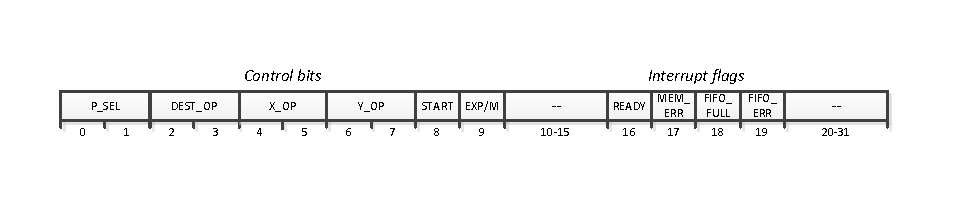
\includegraphics[trim=1.2cm 1.2cm 1.2cm 1.2cm, width=15cm]{pictures/plb_control_reg.pdf}
\caption{control register}
\end{figure}


\begin{tabular}{ll}
bits 0-1 	& P\_SEL : selects which pipeline part to be active\\
 			& $\bullet$  "01" lower pipeline part\\
 			& $\bullet$  "10" higher pipeline part\\
 			& $\bullet$  "11" full pipeline\\
 			& $\bullet$  "00" invalid selection\\
 			&\\
bits 2-3 	& DEST\_OP : selects the operand (0-3) to store the result in for a single\\
 			& Montgomery multiplication\footnotemark\\
 			&\\
bits 4-5 	& X\_OP : selects the x operand (0-3) for a single Montgomery multiplication\footnotemark[\value{footnote}]\\
			&\\
bits 6-7 	& Y\_OP : selects the y operand (0-3) for a single Montgomery multiplication\footnotemark[\value{footnote}]\\
			&\\
bit 8 		& START : starts the multiplication/exponentiation\\
			&\\
bit 9 		& EXP/M : selects the operating mode\\
 			& $\bullet$  "0" single Montgomery multiplications\\
 			& $\bullet$  "1" simultaneous exponentiations\\
 			&\\
bits 10-15	& unimplemented\\
			&\\
bit 16		& READY : ready flag, "1" when multiplication is done\\
			& must be cleared in software\\
			&\\
bit 17		& MEM\_ERR : memory collision error flag, "1" when write error occurred\\
			& must be cleared in software\\
			&\\
bit 18		& FIFO\_FULL : FIFO full error flag, "1" when FIFO is full\\
			& must be cleared in software\\
			&\\
bit 19		& FIFO\_ERR : FIFO write/push error flag, "1" when push error occurred\\
			& must be cleared in software\\
			&\\
bits 20-31	& unimplemented\\
			&\\
\end{tabular}
\newline
\newline
\footnotetext{when the core is running in exponentiation mode, the parameters DEST\_OP, X\_OP and Y\_OP have no effect.}

\newpage
\subsection{Software reset register (offset = 0x0100)}
This is a register with write only access, and provides the possibility to reset the IP core from software by writing
0x0000000A to this address. The reset affects the full IP core, thus resetting the control register, interrupt controller,
the multiplier pipeline, FIFO and control logic of the core.

\subsection{Global interrupt enable register (offset = 0x021C)}
This register contains a single defined bit in the high-order position. The GIE bit enables or disables all interrupts
form the IP core.\\
\begin{figure}[H]
\centering
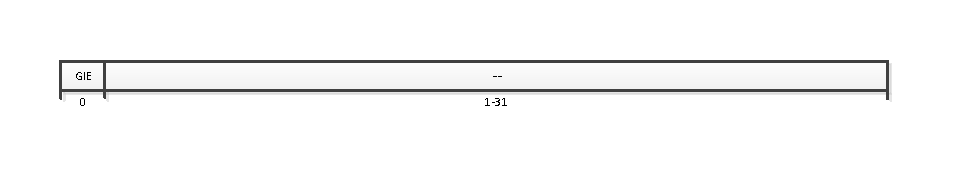
\includegraphics[trim=1.2cm 1.2cm 1.2cm 1.2cm, width=15cm]{pictures/plb_gie_reg.pdf}
\caption{Global interrupt enable register}
\end{figure}

\begin{tabular}{ll}
bit 0 		& GIE : Global interrupt enable\\
 			& $\bullet$  "0" disables all core interrupts\\
 			& $\bullet$  "1" enables all core interrupts\\
 			&\\
bits 1-31	& unimplemented\\
			&\\
\end{tabular}

\subsection{Interrupt status register (offset = 0x0220)}
Read-only register that contains the status of the core interrupts. Currently there is only one common interrupt from
the core that is asserted when a multiplication/exponentiation is done, FIFO is full, on FIFO push error or memory write
collision.\\
\begin{figure}[H]
\centering
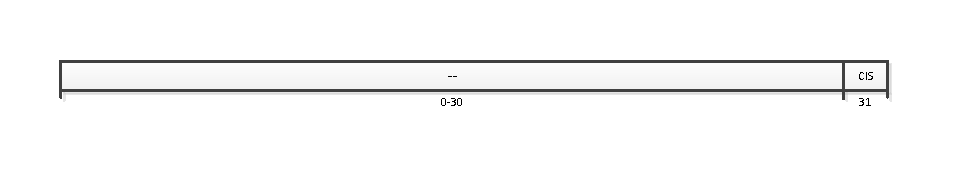
\includegraphics[trim=1.2cm 1.2cm 1.2cm 1.2cm, width=15cm]{pictures/plb_is_reg.pdf}
\caption{Interrupt status register}
\end{figure}

\begin{tabular}{ll}
bits 0-30	& unimplemented\\
			&\\
bit 31 		& CIS : Core interrupt status\\
 			& is high when interrupt is requested from core\\
 			&\\
\end{tabular}

\subsection{interrupt enable register (offset = 0x0228)}
This register contains the interrupt enable bits for the respective interrupt bits of the interrupt status register.\\
\begin{figure}[H]
\centering
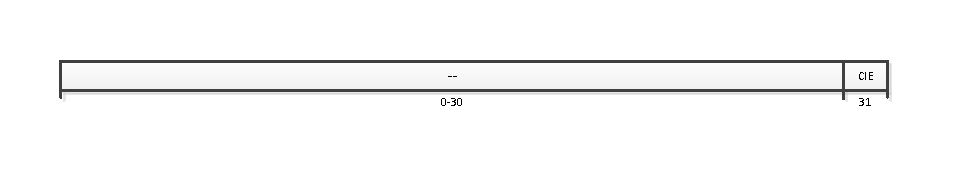
\includegraphics[trim=1.2cm 1.2cm 1.2cm 1.2cm, width=15cm]{pictures/plb_ie_reg.pdf}
\caption{Interrupt enable register}
\end{figure}
\begin{tabular}{ll}
bits 0-30	& unimplemented\\
			&\\
bit 31 		& CIE : Core interrupt enable\\
 			& $\bullet$  "0" disable core interrupt\\
 			& $\bullet$  "1" enable core interrupt\\
 			&\\
\end{tabular}

\section{Interfacing the core's RAM}
Special attention must be taken when writing data to the operands and modulus. The least significant bit of the data has be on the lowest
address and the most significant bit on the highest address. A write to the RAM has to happen 1 word at a time, byte writes are not
supported due to the structure of the RAM.

\section{Handling interrupts}
When the embedded processor receives an interrupt signal from this core, it is up to the controlling software to
determine the source of the interrupt by reading out the interrupt flag of the control register.
\chapter{AXI4-Lite interface}
\section{Structure}
The AXI4-Lite interface for this core acts as a slave to the AXI bus. It only supports the AXI-Lite procotol since there
is no ID reflection of the data transfer and only a 32-bit wide bus is supported. The AXI4-Lite IPcore block contains the
exponentiation core and a control register for the core its control inputs and outputs.

\section{Parameters}
This section describes the parameters used to configure the core, only the relevant parameters are discussed. AXI
specific parameters are left to the user to configure. The IP core specific parameters and their respective use are
listed in the table below.
\begin{center}
	\begin{tabular}{|l|p{6.5cm}|c|l|}
		\hline
		\rowcolor{Gray}
		\textbf{Name} & \textbf{Description} & \textbf{VHDL Type} &\textbf{Default Value} \bigstrut\\
		\hline
		\multicolumn{4}{|l|}{\textit{\textbf{Memory configuration}}} \\		
		\hline
		\verb|C_FIFO_DEPTH| & depth of the generic FIFO, only applicable if \verb|C_MEM_STYLE| = \verb|"generic"| or \verb|"asym"|  & integer & 32 \bigstrut\\
		\hline
		\verb|C_MEM_STYLE| & the memory structure to use for the RAM, choice between 3 options: & string & \verb|"generic"| \bigstrut\\
							& \verb|"xil_prim"| : use xilinx primitives & & \\
      						& \verb|"generic"| : use general 32-bit RAMs & & \\
      						& \verb|"asym"| : use asymmetric RAMs & & \\
      						& (For more information see \ref{subsec:RAM_and_FIFO}) & & \bigstrut[b] \\
		\hline
		\verb|C_FPGA_MAN| & device manufacturer: & string & \verb|"xilinx"| \\
						& \verb|"xilinx"| or \verb|"altera"| &  &  \bigstrut\\
		\hline
		\verb|C_BASEADDR| & base address for the IP core's memory space & std\_logic\_vector & X"FFFFFFFF" \bigstrut\\
		\hline
		\verb|C_HIGHADDR| & high address for the IP core's memory space & std\_logic\_vector & X"00000000" \bigstrut\\
		\hline
		\multicolumn{4}{|l|}{\textit{\textbf{Multiplier configuration}}} \\
		\hline
		\verb|C_NR_BITS_TOTAL| & total width of the multiplier in bits & integer & 1536\bigstrut\\
		\hline
		\verb|C_NR_STAGES_TOTAL| & total number of stages in the pipeline & integer & 96\bigstrut\\
		\hline
		\verb|C_NR_STAGES_LOW| & number of lower stages in the pipeline, defines the bit-width of the lower pipeline part & integer & 32 \bigstrut\\
		\hline
		\verb|C_SPLIT_PIPELINE| & option to split the pipeline in 2 parts & boolean & true \bigstrut\\
		\hline
	\end{tabular}%
\end{center}
%\newline 
\newpage
The IP core's memory space is organised in a fixed structure as show in Figure~\ref{AXImemstructure}. Only the upper 17
bits (31:15) of the base address can be chosen freely, the lower bits must be 0. So the \verb|C_BASEADDR| parameter must end
in 0xXXXX0000 or 0xXXXX8000 in hexadecimal representation. The core's memory space must have a minimum width of 28K byte for 
all registers to be accessible.
\begin{figure}[H]	
\centering
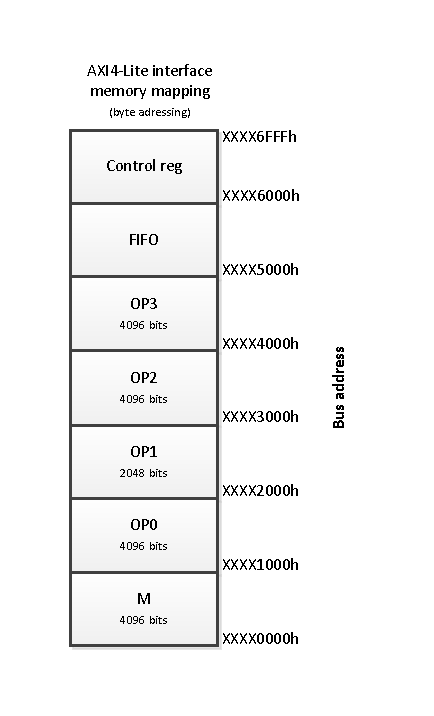
\includegraphics[trim=1.2cm 1.2cm 1.2cm 1.2cm, width=5cm]{pictures/axi_mem.pdf}
\caption{AXI4-Lite IP core memory structure}
\label{AXImemstructure}
\end{figure}

There are 4 parameters to configure the multiplier. These values define the width of the multiplier operands and the
number of pipeline stages. If \verb|C_SPLIT_PIPELINE| is false, only operands with a width of\\\verb|C_NR_BITS_TOTAL| are
valid. Else if \verb|C_SPLIT_PIPELINE| is true, 3 operand widths can be supported:
\begin{itemize}
  \item the length of the full pipeline ($C\_NR\_BITS\_TOTAL$)
  \item the length of the lower pipeline ($\frac{C\_NR\_BITS\_TOTAL}{C\_NR\_STAGES\_TOTAL} \cdot C\_NR\_STAGES\_LOW $)
  \item the length of the higher pipeline ($\frac{C\_NR\_BITS\_TOTAL}{C\_NR\_STAGES\_TOTAL} \cdot (C\_NR\_STAGES\_TOTAL - C\_NR\_STAGES\_LOW$)
\end{itemize}

\section{IO ports}
\begin{tabular}{|l|c|c|l|}
	\hline
	\rowcolor{Gray}
	\textbf{Port} & \textbf{Width} & \textbf{Direction} & \textbf{Description} \\
	\hline
	\multicolumn{4}{|l|}{\textit{\textbf{AXI4-Lite bus connections}}} \\
	\hline
	\verb|S_AXI_ACLK| & 1     & in & see note 1 \\
	\hline
	\verb|S_AXI_ARESETN| & 1     & in & see note 1 \\
	\hline
	\verb|S_AXI_AWADDR| & 32    & in & see note 1 \\
	\hline
	\verb|S_AXI_AWVALID| & 1     & in & see note 1 \\
	\hline
	\verb|S_AXI_AWREADY| & 1     & out & see note 1 \\
	\hline
	\verb|S_AXI_WDATA| & 32     & in & see note 1 \\
	\hline
	\verb|S_AXI_WVALID| & 1     & in & see note 1 \\
	\hline
	\verb|S_AXI_WREADY| & 1     & out & see note 1 \\
	\hline
	\verb|S_AXI_WSTRB| & 4     & in & see note 1 \\
	\hline
	\verb|S_AXI_BVALID| & 1    & out & see note 1 \\
	\hline
	\verb|S_AXI_BREADY| & 1     & in & see note 1 \\
	\hline
	\verb|S_AXI_BRESP| & 2     & out & see note 1 \\
	\hline
	\verb|S_AXI_ARADDR| & 32     & in & see note 1 \\
	\hline
	\verb|S_AXI_ARVALID| & 1     & in & see note 1 \\
	\hline
	\verb|S_AXI_ARREADY| & 1     & out & see note 1 \\
	\hline
	\verb|S_AXI_RDATA| & 32     & out & see note 1 \\
	\hline
	\verb|S_AXI_RVALID| & 1    & out & see note 1 \\
	\hline
	\verb|S_AXI_RREADY| & 1     & in & see note 1 \\
	\hline
	\verb|S_AXI_RRESP| & 2     & out & see note 1 \\
	\hline
	\multicolumn{4}{|l|}{\textit{\textbf{Core signals}}} \\
	\hline
	\verb|IntrEvent| & 1     & out   & core interrupt signal \\
	\hline
	\verb|calc_time| & 1     & out   & is high when core is performing a multiplication, for monitoring \\
	\hline
\end{tabular}%
\newline \newline
\textbf{Note 1:} The function and timing of this signal is defined in the AMBA\textsuperscript{\textregistered} AXI Protocol Version: 2.0 Specification.

\section{Registers}
This section specifies the IP core internal registers as seen from the software. These registers allow to control and
configure the modular exponentiation core and to read out its state. All addresses given in this table are relative to the
IP core's base address.\\
\newline
% Table generated by Excel2LaTeX
\begin{tabular}{|l|c|c|c|l|}
\hline
\rowcolor{Gray}
\textbf{Name} & \textbf{Width} & \textbf{Address} & \textbf{Access} & \textbf{Description} \bigstrut\\
\hline
control register 		& 32 & 0x6000 & RW 	& multiplier core control signals and \bigstrut[t]\\
						&	&		&		& interrupt flags register\bigstrut[b]\\
\hline
\end{tabular}%
\newpage
\subsection{Control register (offset = 0x6000)}
This registers holds the control inputs to the multiplier core and the interrupt flags.\\
\begin{figure}[H]
\centering
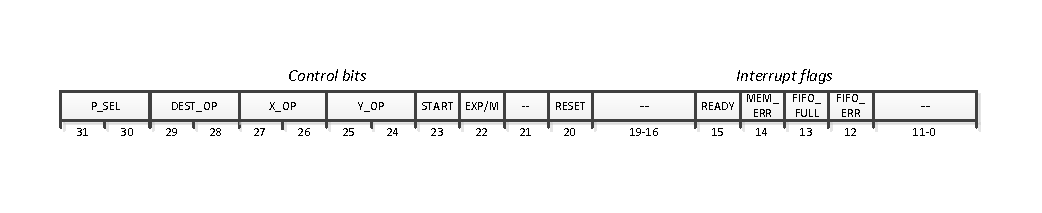
\includegraphics[trim=1.2cm 1.2cm 1.2cm 1.2cm, width=15cm]{pictures/axi_control_reg.pdf}
\caption{control register}
\end{figure}

\begin{tabular}{ll}
bits 31-30 	& P\_SEL : selects which pipeline part to be active\\
 			& $\bullet$  "01" lower pipeline part\\
 			& $\bullet$  "10" higher pipeline part\\
 			& $\bullet$  "11" full pipeline\\
 			& $\bullet$  "00" invalid selection\\
 			&\\
bits 29-28 	& DEST\_OP : selects the operand (0-3) to store the result in for a single\\
 			& Montgomery multiplication\footnotemark\\
 			&\\
bits 27-26 	& X\_OP : selects the x operand (0-3) for a single Montgomery multiplication\footnotemark[\value{footnote}]\\
			&\\
bits 25-24 	& Y\_OP : selects the y operand (0-3) for a single Montgomery multiplication\footnotemark[\value{footnote}]\\
			&\\
bit 23 		& START : starts the multiplication/exponentiation\\
			&\\
bit 22 		& EXP/M : selects the operating mode\\
 			& $\bullet$  "0" single Montgomery multiplications\\
 			& $\bullet$  "1" simultaneous exponentiations\\
 			&\\
bit 21		& unimplemented\\
			&\\
bit 20 		& RESET : active high reset for the core\footnotemark[2]\\
			&\\		
bits 19-16	& unimplemented\\
			&\\
bit 15		& READY : ready flag, "1" when multiplication is done\\
			& must be cleared in software\\
			&\\
bit 14		& MEM\_ERR : memory collision error flag, "1" when write error occurred\\
			& must be cleared in software\\
			&\\
bit 13		& FIFO\_FULL : FIFO full error flag, "1" when FIFO is full\\
			& must be cleared in software\\
			&\\
bit 12		& FIFO\_ERR : FIFO write/push error flag, "1" when push error occurred\\
			& must be cleared in software\\
			&\\
bits 11-0	& unimplemented\\
			&\\
\end{tabular}
\newline
\newline
\footnotetext[1]{when the core is running in exponentiation mode, the parameters DEST\_OP, X\_OP and Y\_OP have no effect.}
\footnotetext[2]{The reset affects the full IP core, thus resetting the control register, interrupt controller,
the multiplier pipeline, FIFO and control logic of the core.}
\newpage
\section{Interfacing the core's RAM}
Special attention must be taken when writing data to the operands and modulus. The least significant bit of the data has be on the lowest
address and the most significant bit on the highest address. A write to the RAM has to happen 1 word at a time, byte writes are not
supported due to the structure of the RAM.

\section{Handling interrupts}
When the embedded processor receives an interrupt signal from this core, it is up to the controlling software to determine the source of the interrupt by reading out the interrupt flags of the control register. After handling the interrupt, the appropriate flag must be cleared by user. A reset or core start operation also resets the flags. The interrupt signal is high level sensitive.
\chapter{Performance and resource usage}

This Modular Simultaneous Exponentiation IP core is designed to speed up modular simultaneous exponentiations on embedded systems.
On embedded processors, software implementations (even with specialized libraries like GMP\footnote{GNU Multiple Precision Arithmetic Library -- Project website: \url{http://gmplib.org/}}), demand much CPU time when large operands are used.
Practical tests of this core have shown a significant speed-up compared to software computations. For $n=1536$ and $t=1024$, hardware is about 70 times faster than a GMP-based implementation (with embedded linux) an a 100 MHz MicroBlaze processor (32-bit).\\

For the multiplier, execution time is given by~(\ref{eq:Tmult}), where $\tau_c$ is defined by the core operating
frequency. Since the maximum frequency is highly influenced by the latency in the critical path, we can expect to
achieve higher frequencies for shorter stage lengths. This trend is seen in Figure~\ref{fig:Virtex6exctime} for
different operand lengths, which are results used from the static timing analysis during synthesis. A minimum execution
time in this graph is found when the maximum operating frequency of the core first reaches the maximum frequency of the
FGPA in use. Beyond that point, using a smaller stage width has no positive effect anymore because the frequency can not
rise anymore and the number of clock cycles to complete a multiplication increases. Another remark that can be made is
that splitting the pipeline, has no considerable effect on the performance of the core.

\begin{figure}[H]
\centering
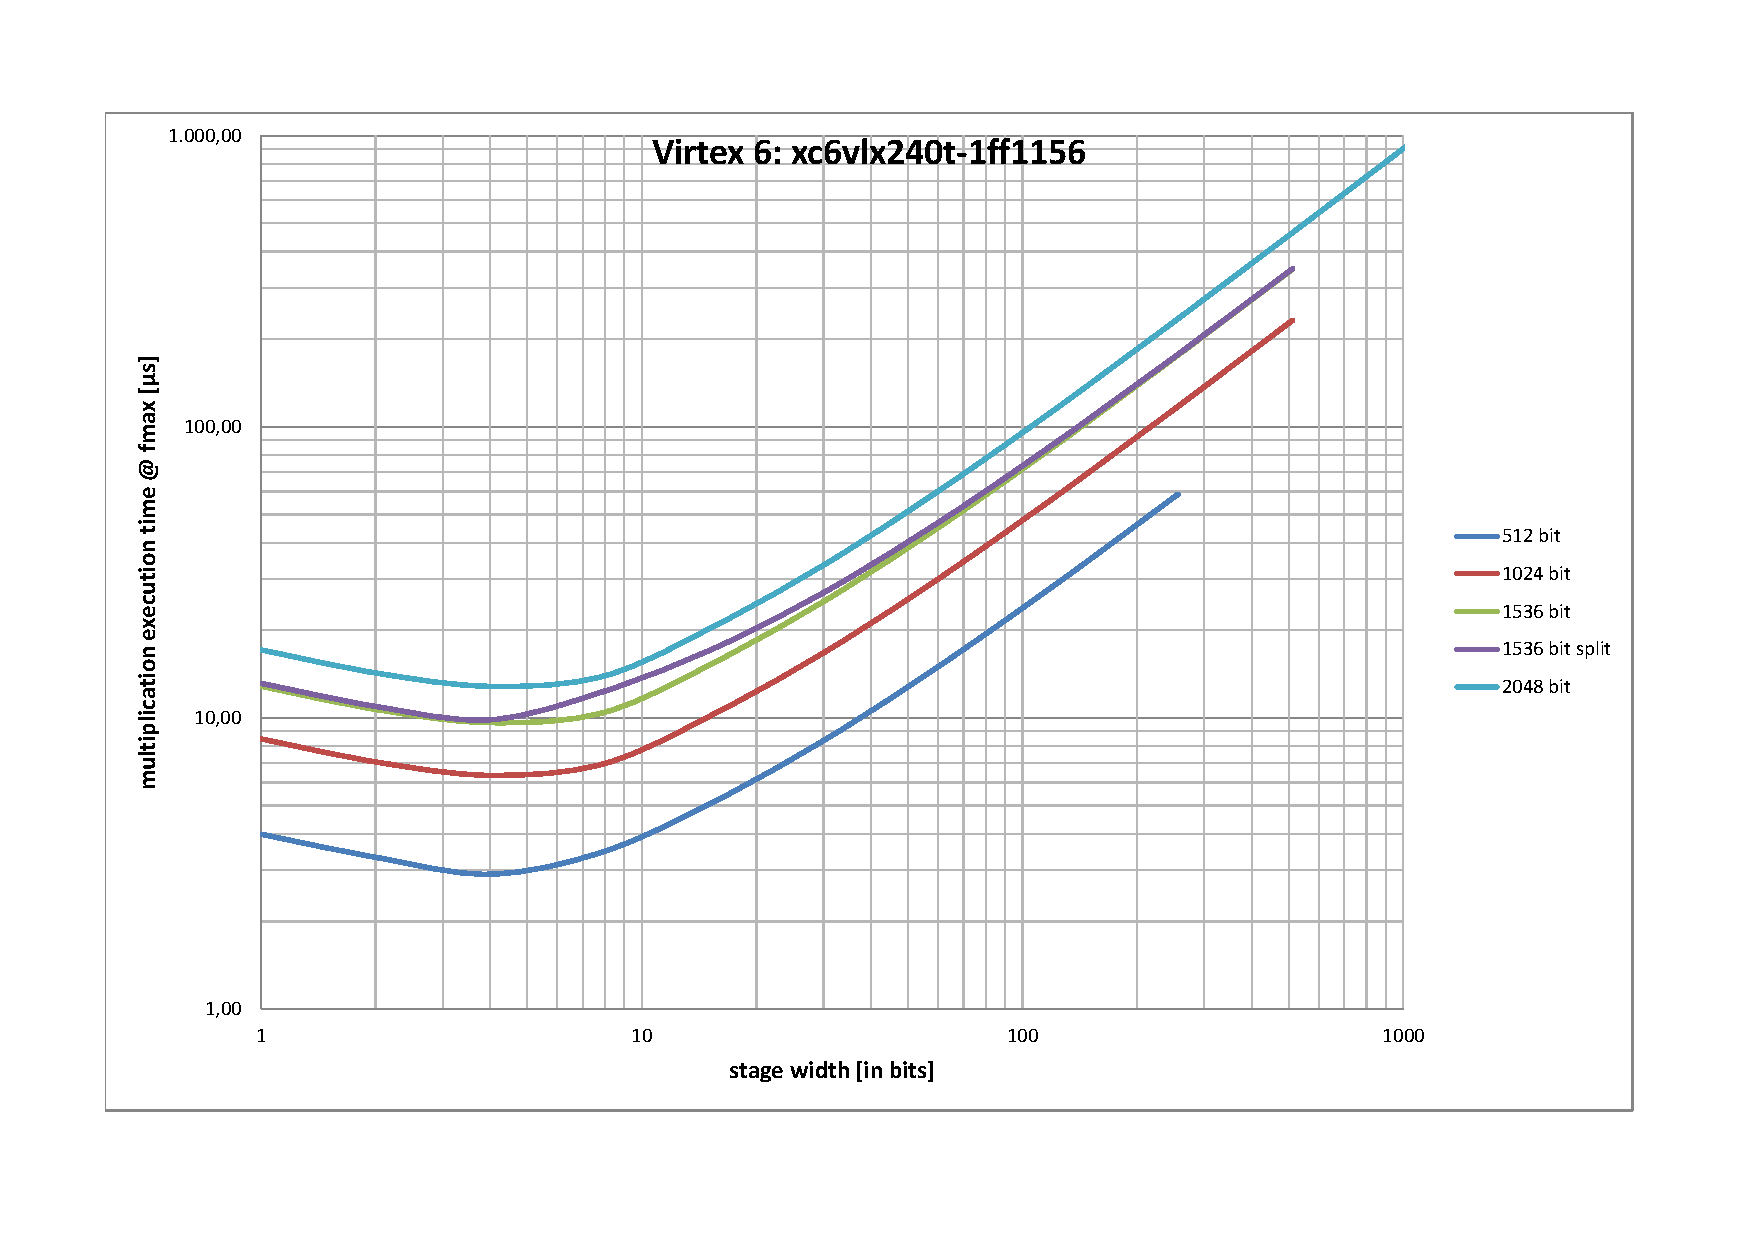
\includegraphics[trim=2cm 2cm 2cm 2cm, width=16cm]{pictures/Virtex6_stagewidth.pdf}
\caption{Example of multiplication execution time in function of the stage width for a Virtex6 FPGA.}
\label{fig:Virtex6exctime}
\end{figure}

In general, shorter stage lengths result in smaller execution times. However, using more stages implies that more
flip-flops will be needed, thus more resources are used. A balance must be found between a execution time and resources.
Currently, the core's operating frequency is the same as the bus frequency of the embedded processor. For optimal
operation of the core, the stage width must be chosen so that the maximum frequency given in synthesis is just above or
equal to the bus frequency.

In the tables below resource usage and timing results are shown for different operand lengths and FPGA's. As a rule of thumb, the number of flip-flops is given by~(\ref{eq:ff}).
\begin{align}\label{eq:ff}
5+2\cdot n+6\cdot\frac{n}{s}+\lceil\log_{2}(n)\rceil+\lceil\log_{2}(\frac{n}{s})\rceil
\end{align}
where $s$ is the stage width.

The number of LUTs is almost completely determined by $n$ and the number of LUT-inputs. A pre-synthesis estimate can be made with~(\ref{eq:lut4}) and~(\ref{eq:lut6}).
\begin{align}
8\cdot n \hspace{1cm}\text{for 4-input LUTs} \label{eq:lut4}\\
6\cdot n \hspace{1cm}\text{for 6-input LUTs} \label{eq:lut6}
\end{align}
\newline

Results for a Virtex 6 device xc6vlx240t-1ff1156, speedgrade -1\\
Synthesis settings: Optimization: area, Effort: high\\
% Table generated by Excel2LaTeX from sheet 'Virtex 6'
\begin{tabular}{rcccccccccccc}
\hline
\hline
$n$     & \multicolumn{3}{c}{512} &       & \multicolumn{3}{c}{1024} &       & \multicolumn{3}{c}{2048} & [bit] \bigstrut[t]\\
$stage width$ & 64    & 16    & 4     &       & 64    & 16    & 4     &       & 64    & 16    & 4     & [bit] \bigstrut[b]\\
\hline
$f_{max}$  & 64,91 & 199,96 & 395,57 &       & 64,91 & 199,66 & 358,62 &       & 94,91 & 199,96 & 358,62 & [MHz] \bigstrut[t]\\
$T_m@f_{max}$ & 15,87 & 5,27  & 2,91  &       & 31,77 & 10,55 & 9,63  &       & 63,57 & 21,11 & 12,84 & [$\mu$s] \\
$cycles$ & 1030  & 1054  & 1150  &       & 2062  & 2110  & 3454  &       & 4126  & 4222  & 4606  & [cycles] \\
\textbf{Resources} &       &       &       &       &       &       &       &       &       &       &       &  \\
Flipflops & 1089  & 1235  & 1813  &       & 2163  & 2453  & 5401  &       & 4309  & 4887  & 7193  &  \\
LUT's & 3094  & 3096  & 3102  &       & 6169  & 6171  & 9252  &       & 12315 & 12318 & 12324 &  \bigstrut[b]\\
\hline
\hline
\end{tabular}%
\vspace{1cm}
\newline
Results for a Spartan 3 device xc3s1000-5fg320, speedgrade -5\\
Synthesis settings: Optimization: area, Effort: high\\
% Table generated by Excel2LaTeX from sheet 'Spartan 3'
\begin{tabular}{rccccccccc}
\hline
\hline
$n$     & \multicolumn{3}{c}{256} & & \multicolumn{4}{c}{512}       & [bit] \bigstrut[t]\\
$stage width$ & 32    & 8     & 2    & & 64    & 32    & 8     & 2     & [bit] \bigstrut[b]\\
\hline
$f_max$  & 21,49 & 69,30 & 127,32 & & 11,36 & 21,49 & 69,30 & 127,32 & [MHz] \bigstrut[t]\\
$T_m@f_{max}$ & 24,1  & 7,82  & 5,01  & & 90,7  & 48,29 & 15,67 & 10,04 & [$\mu$s] \\
$cycles$ & 518   & 542   & 638 &  & 1030  & 1038  & 1086  & 1278  & [cycles] \\
\textbf{Resources} &       &    &   &       &       &       &       &       &  \\
Flipflops & 576   & 722   & 1300 & & 1089  & 1138  & 1428  & 2582  &  \\
LUT's & 2072  & 2074  & 2079 & & 4124  & 4126  & 4128  & 4135  &  \bigstrut[b]\\
\hline
\hline
\end{tabular}%
\vspace{1cm}
\newline
Results for a Virtex 4 device xc4vlx200-11ff1513, speedgrade -11\\
Synthesis settings: Optimization: area, Effort: high\\
% Table generated by Excel2LaTeX from sheet 'Virtex 4'
\begin{tabular}{rcccccccccc}
\hline
\hline
$n$     & \multicolumn{4}{c}{512}    &   & \multicolumn{4}{c}{1024}      & [bit] \bigstrut[t]\\
$stage width$ & 64    & 32    & 8     & 2    & & 128   & 32    & 8     & 2     & [bit] \bigstrut[b]\\
\hline
$f_{max}$  & 22,83 & 43,05 & 138,31 & 246,98 & & 11,77 & 43,05 & 138,31 & 246,98 & [MHz] \bigstrut[t]\\
$T_m@f_{max}$ & 45,12 & 24,11 & 7,85  & 5,17 & & 87,5  & 24,5  & 8,31  & 6,21  & [$\mu$s] \\
$cycles$ & 1030  & 1038  & 1086  & 1278 & & 1030  & 1054  & 1150  & 1534  & [cycles] \\
\textbf{Resources} &  &       &       &     &  &       &       &       &       &  \\
Flipflops & 1089  & 1138  & 1428  & 2582 & & 2114  & 2260  & 2838  & 5144  &  \\
LUT's & 4124  & 4126  & 4128  & 4135 & & 8225  & 8230  & 8234  & 8238  &  \bigstrut[b]\\
\hline
\hline
\end{tabular}%



\bibliography{cited}

\chapter*{License}
Copyright (C) 2011 DraMCo research group and OPENCORES.ORG \\This project may be used and distributed without restriction
provided that the copyright statement is not removed from the files and that any derivative work contains the original
copyright notice and the associated disclaimer.\\
 
This project is free software; you can redistribute it and/or modify it under the terms of the GNU Lesser General Public
License as published by the Free Software Foundation; either version 2.1 of the License, or (at your option) any later
version.\\
 
This project is distributed in the hope that it will be useful, but WITHOUT ANY WARRANTY; without even the implied
warranty of MERCHANTABILITY or FITNESS FOR A PARTICULAR PURPOSE. See the GNU Lesser General Public License for more
details.\\

You should have received a copy of the GNU Lesser General Public License along with this source; if not, download it
from http://www.opencores.org/lgpl.shtml
\end{document}
